In this chapter, we discuss three studies to evaluate various aspects of \Edgeworth (\cref{chp:edgeworth}). To effectively scale up visual practice authoring, \Edgeworth must support a diverse set of instructional domains, generate high-quality diagrams consistently, and allow educators to author real-world problems. In \cref{sec:edgeworth-user-study,sec:reliability-eval,sec:expert-feedback}, we evaluate \Edgeworth by answering the following research questions on these qualities:

\begin{itemize}
    \item\textbf{Reliability} (\ref{rq:mut}): Can \Edgeworth reliably generate translation problems with relatively few variations required?
    \item\textbf{Efficiency} (\ref{rq:eff}): comparing with a conventional drawing tool, are authors more efficient at making translation problems using \Edgeworth? 
    \item\textbf{Ecological validity} (\ref{rq:eco}): Do real-world instructors consider \Edgeworth-generated translation problems to be useful? 
\end{itemize}

First, we evaluated the reliability of \Edgeworth by labeling 310 diagram variations from translation problem dataset (\cref{sec:edgeworth-case-studies}) by hand. With high inter-rater reliability, the result shows that \Edgeworth can reliably generate diagrams that constitute valid four-choice translation problems, when constrained to 10 variations per problem.

Second, we performed a usability evaluation of \Edgeworth to measure authors' efficiency at creating translation problems compared with a conventional drawing tool. The results show that authors are about 3 times faster at making diagrammatic options for translation problems using \Edgeworth compared to Google Drawings. 

Finally, we conducted walkthrough demonstrations with 9 educators that have experience creating problems. The goal of the demonstrations was to obtain feedback on the ecological validity of \Edgeworth-generated problems and the usefulness of \Edgeworth in general. Overall, these experts found \Edgeworth-generated problems to contain pedagogically useful variations and high visual quality. They provided detailed feedback on individual diagram variations and suggested how \Edgeworth might fit into their instructional contexts. 

\section{Reliability Evaluation (\ref{rq:mut})}
\label{sec:reliability-eval}

\Edgeworth's approach involves random mutations. The mutation operations are type-safe, but type-safety does not prevent degenerate diagram layouts. For instance, \sub{Point A, B} followed by \sub{Triangle t := MkTriangle(A, A, B)} will typecheck. However, since the triangle described in this scenario involves the \sub{Point A} twice, \Edgeworth will produce a line segment, not a triangle from this scenario. Are \Edgeworth suggestions dominated by these nonsensical scenarios? In this section, we evaluate whether \Edgeworth can reliably suggest diagrams that are valid answer options to multiple-choice translation problems (\ref{rq:mut}). 

\subsection{Methods}
\label{sec:reliability-method}

The goal of \Edgeworth is to generate enough diagram variations to assemble a four-choice multiple-choice problem for a given prompt. To this end, we use the following classification scheme for diagram variations: a variation can be a \textbf{Correct} or \textbf{Incorrect} answer to the prompt, or \textbf{Discard}ed because the diagram is invalid for missing key components or lacking readability.

For \ref{rq:mut}, we define ``relatively few variations'' to be 10 diagrams, and consider \Edgeworth to have generated a translation problem in $n$ variations if at that point we have (possibly including the original diagram) at least one \textbf{Correct} diagram, at least one \textbf{Incorrect} diagram, and in total at least four diagrams that are either \textbf{Correct} or \textbf{Incorrect}.

To evaluate this coding scheme, we randomly sampled 2 problems from each of our 3 domains, for 60 generated diagrams total. The first two authors each coded all 60 of those sample diagrams, after which we calculated the Cohen's $\kappa$ \cite{cohen1960coefficient} statistic. Then with the assumption that our coding scheme has reasonable inter-rater reliability, at least one author coded all remaining diagrams, allowing us to determine the number of our prompts for which \Edgeworth was able to successfully generate a multiple-choice problem. The coding results are included in supporting files.

\subsection{Results}

\subsubsection{Reliability of problem generation}

For \ref{rq:mut}, we found that \Edgeworth generated valid multiple-choice problems for 27/31 prompts within 10 variations, and for 30/31 problems within 20 variations. For each of these four failures with 10 variations, \Edgeworth did generate at least four \textbf{Correct} examples, but we had to \textbf{Discard} all the other diagrams, leaving no \textbf{Incorrect} examples. For the one remaining failure with 20 variations, \Edgeworth never succeeded even after we increased the number of variations to 50.


\subsubsection{Distribution}

\begin{table}
    \centering
    \begin{tabular}{r|rrr|r}
        & \textbf{Correct} & \textbf{Incorrect} & \textbf{Discard} & \textit{total} \\
        \hline
        geometry & 52 & 54 & 64 & 170 \\
        chemistry & 3 & 54 & 13 & 70 \\
        discrete & 28 & 25 & 17 & 70 \\
        \hline
        \textit{total} & 85 & 133 & 94 & 310
    \end{tabular}
    \caption{Distribution of diagram variation classes.}
    % \Description{This table describes the coding results from the reliability evaluation. There are four rows (blank, geometry, chemistry, discrete, and total) and five columns (blank, correct, incorrect, discard, and total). The first row and first column contain the headers. The numbers starting from row 2, column 2, in row order are: Row 2: 52, 54, 64, 170; Row 3: 3, 54, 13, 70; Row 4: 28, 25, 17, 70; Row 5: 85, 133, 94, 310}
    \label{tab:distribution}
\end{table}

The original diagram is a \textbf{Correct} answer for every prompt, except for the two Euler circuit prompts, in which the original diagram is \textbf{Incorrect}. For \Edgeworth-generated variations, the full distribution of classes is shown in Table~\ref{tab:distribution}.

The chemistry domain had a far smaller proportion of \textbf{Correct} variations than the other two domains because the only way for a variation to be \textbf{Correct} is for it to coincidentally be identical to the original diagram. Interestingly, in the other two domains, there were about the same number of \textbf{Correct} and \textbf{Incorrect} variations.

In the geometry domain, \textbf{Discard}ed diagrams were primarily either diagrams missing elements referred to in the question prompt, or diagrams that were visually degenerate (\eg everything compressed into a single line). In chemistry, we \textbf{Discard}ed diagrams where the molecule was disconnected. Finally, in the graph domain, we \textbf{Discard}ed diagrams in which some nodes were labeled and others were unlabeled (\ie \Edgeworth had inserted new unlabeled nodes when all nodes in the original diagram were labeled).

\subsubsection{Inter-rater Agreement}

We sampled two problems per domain from the problems collected in ~\cref{sec:edgeworth-case-studies} to evaluate inter-rater agreement (six problems or sixty diagrams in total, 19\% of the dataset). We found perfect agreement on that sample, so $\kappa = 1$.

\section{Experimental Evaluation of Authoring Efficiency (\ref{rq:eff})}
\label{sec:edgeworth-user-study}

To answer \ref{rq:eff}, we conduct an experiment that compares \Edgeworth against a conventional drawing tool in translation problem authoring tasks. In this section, we describe the experimental setup and findings.

\subsection{Study Design}


\subsubsection{Participants}

We recruited 16 participants through advertisement in the university community (e.g. emails and Slack channels). Participants were screened to have some past experience using digital drawing tools. All participants reported that they have used Google Drawings and/or equivalent tools to make diagrams in the past.

\subsubsection{Tasks}
\label{sec:edgeworth-user-tasks}

\begin{figure}
    \centering
    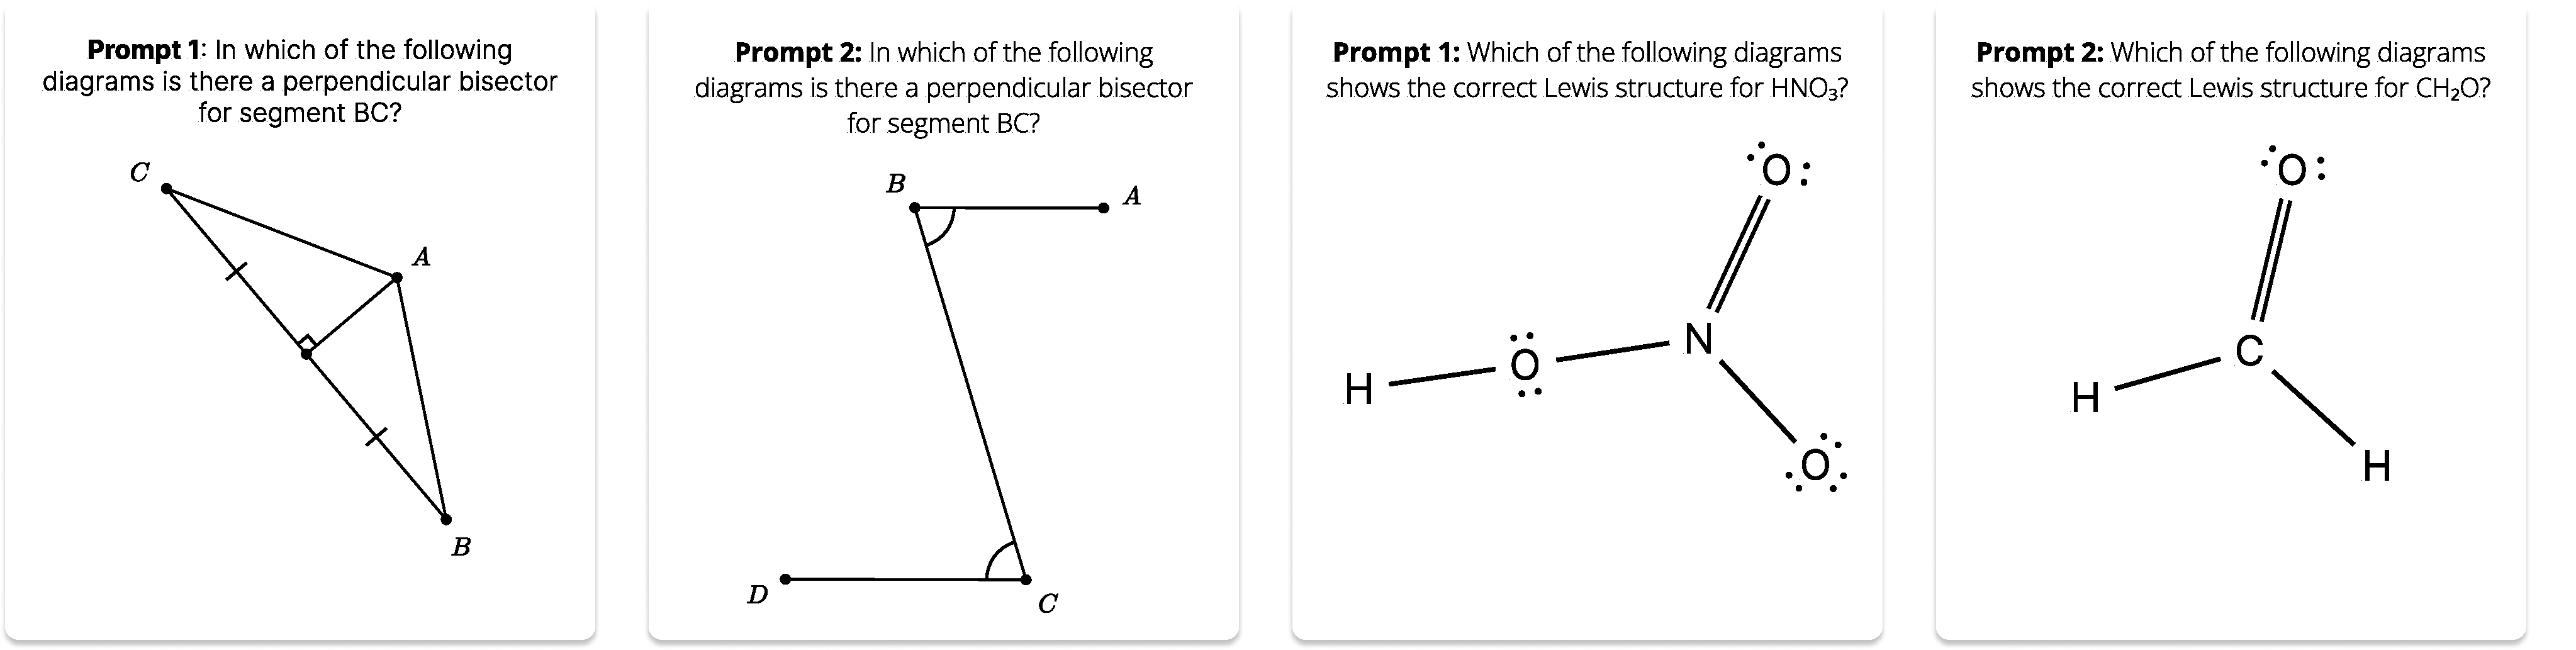
\includegraphics[width=\linewidth]{assets/edgeworth-eval/user-study-tasks.pdf}
    \caption{Tasks used in the \Edgeworth experimental evaluation.}
    \label{fig:edgeworth-user-study-tasks}
\end{figure}

We selected four problem prompts from the translation problem dataset (\cref{sec:edgeworth-case-studies}), two from the chemistry domain and two from geometry, shown in \cref{fig:edgeworth-user-study-tasks}.

We segmented the authoring of the first correct diagram and subsequent incorrect diagrams in the tasks. This segmentation allows us to separately measure the authoring efficiency of creating the example scenario (\cref{sec:create-scenario}) and creating counterexamples (\cref{sec:select-diagrams}). For participants who used \Edgeworth, we were particularly interested in the upfront cost of making the first \Substance diagram in the \Penrose editor. 

For each task, the participant were given (1) a textual problem prompt and (2) an example diagram (\ie a correct response to the prompt). Participants were then given up to 20 minutes to complete each task, which involve two sub-tasks: (a) participants first re-created one example visually similar to the given diagram and then (b) made up to 10 incorrect diagrams by editing the diagram produced in sub-task (a). Each sub-task is time-bounded to 10 minutes. If the participant failed to produce 1 correct diagram in the first segment, they were provided with one so they could continue to the next segment. Each participant completed two problem prompts in chemistry or geometry. 

\subsubsection{Experimental Design}

% groups
The study was a within-subject design, where participants used \Edgeworth and Google Drawings to author diagrams in a counterbalanced order. Participants were further randomly assigned into one of two groups: one group made chemistry diagrams and the second group made geometry diagrams. In the 90-minute study session, each participant was given two problem prompts in total, each repeated twice for \Edgeworth and Google Drawings, so four tasks in total. For instance, a participant in the chemistry-drawing group (first row in \cref{tab:edgeworth-experiment-setup} would spend up to 20 minutes making 1 correct and up to 10 incorrect diagrams of \ensuremath{\mathrm{CH_2O}} using Google Drawings first, and then another 20 minutes on the same prompt using \Penrose and \Edgeworth. After that, this participant would repeat the same for  \ensuremath{\mathrm{HNO_3}}. \cref{tab:edgeworth-experiment-setup} summarizes the four groups resulted from the tool and domain assignments.

\begin{table}
\centering
\begin{tabular}{l|llllll}
Domain & Task 1 (Prompt 1) & Task 2 (Prompt 1) & Task 3 (Prompt 2) & Task 4 (Prompt 2)  \\ \hline
Chemistry &  Google Drawings & \Edgeworth & Google Drawings & \Edgeworth \\
Chemistry & \Edgeworth & Google Drawings & \Edgeworth & Google Drawings \\
Geometry &  Google Drawings & \Edgeworth & Google Drawings & \Edgeworth \\
Geometry & \Edgeworth & Google Drawings & \Edgeworth & Google Drawings \\
\end{tabular}
\label{tab:edgeworth-experiment-setup}
\caption{Participants were divided into 4 groups by the tools they used and diagramming domains of the tasks.}
\end{table}

% authoring assistance

\begin{figure}
    \centering
    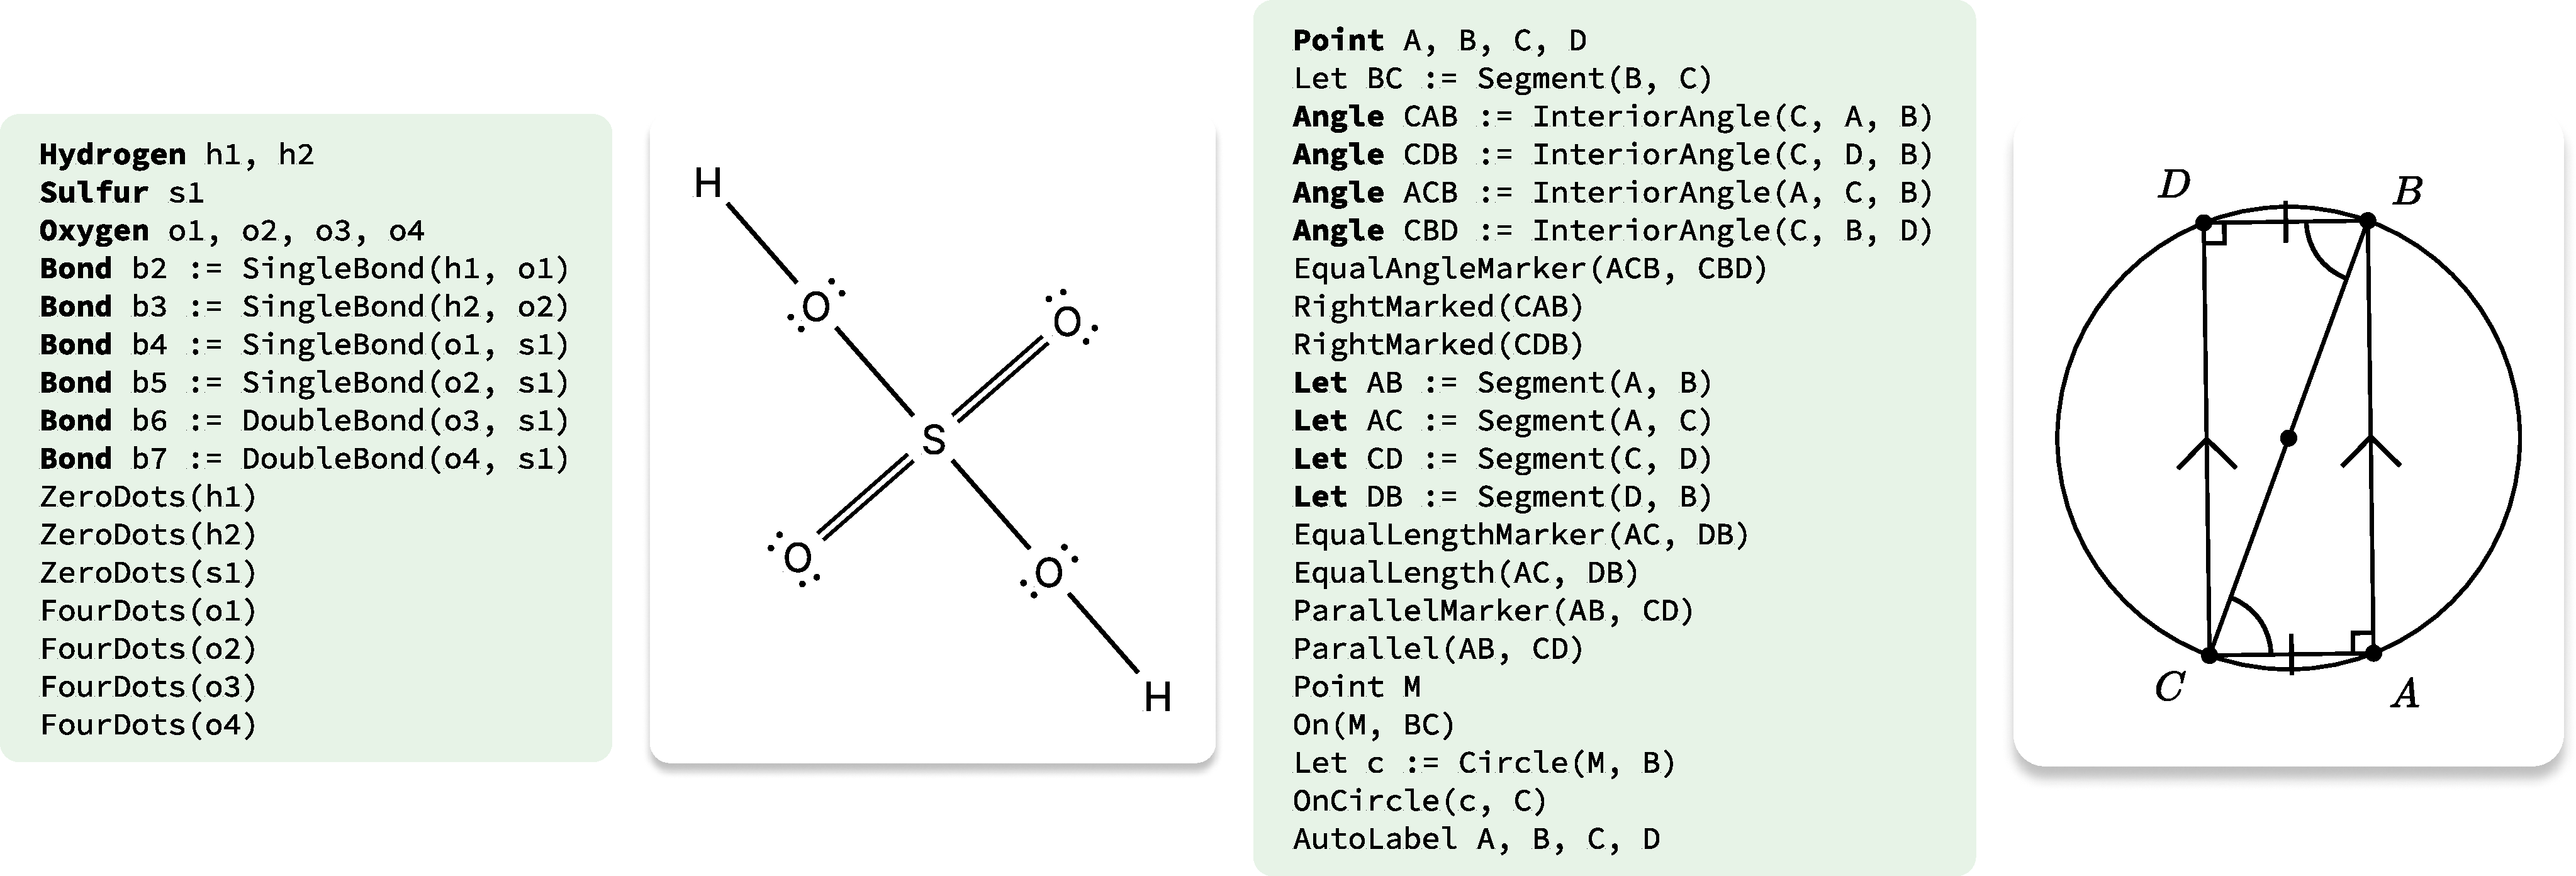
\includegraphics[width=\linewidth]{assets/edgeworth-eval/user-study-examples.pdf}
    \caption{Participants were provided both Google Drawings and \Substance examples throughout the study.}
    \label{fig:edgeworth-user-study-examples}
\end{figure}

At the start of each study session, participants were given 5-minute tutorials of \Edgeworth and Google Drawings, in which they were guided to draw either a right triangle or the Lewis structure of \ensuremath{\mathrm{O_2}}. The ordering of tutorials match the counterbalanced ordering of Google Drawings and \Edgeworth. Throughout the session, participants had access to one Google Drawings example and one \Substance example. \cref{fig:edgeworth-user-study-examples} shows the chemistry and geometry examples. The examples are samples from the translation problem dataset that are visually more complex than the actual study tasks. We provided them to the participants as an authoring aid so that they can copy elements from the examples to save time, analogous to the real-world experience of copying and pasting online examples reported in \cref{sec:edgeworth-formative}.

Participants received no more instructions during the tasks. The experimenter only observed the participant and used a stopwatch to measure the time on task. After completing each task, participants completed a survey that asked them if they agree with the following statements on a 5-point Likert scale:

\begin{itemize}
  \item I would use this problem for a class that I
teach.
  \item The problem is pedagogically useful (\ie students will benefit from doing this problem).  
  \item The diagrams in the problem are of high visual quality.
\end{itemize}

The study took about 90 minutes per participant, using a provided MacBook Pro with the latest version of Chrome installed. The study sessions were audio-recorded and transcribed. All participants were compensated \$25 for their time.

\subsection{Results}

% completion
\cref{tab:edgeworth-user-study-timing} shows the average total time, diagrams produced, and time per diagram for all participants. The \textbf{Diagram Ct} column in \cref{tab:edgeworth-user-study-timing} shows how many diagrams participants produced in each segment of all tasks on average. Any number lower than 1 for correct segments and 10 for incorrect segments indicates that the corresponding participant did not complete the subtask. 
All participants authored 10 incorrect diagrams within 10 minutes using \Edgeworth for both domains. 6 out of 8 participants (11 out of 16 total subtasks) failed to do so using Google Drawings for at least one geometry subtask, and 1 out of 8 participants failed in chemistry. All participants were able to complete the correct diagram for both chemistry prompts using both tools. For the geometry tasks, all participants produced one correct diagram in the first segment using Google Drawings, but 3 failed using \Penrose. 

\begin{table}[h!]
\centering
\begin{tabular}{|l|l|l|r|r|r|}
\hline
\textbf{Domain} & \textbf{Segment} & \textbf{Tool} & \textbf{Total Time} & \textbf{Diagram Ct} & \textbf{Time/Diagram} \\ \hline
Chemistry & correct   & \Penrose        & 144.19s & 1.00  & 144.19s \\ \cline{3-6} 
          &           & Google Drawings & 231.81s & 1.00  & 231.81s \\ \cline{2-6}
          & incorrect & \Edgeworth      & 150.13s & 10.00 & 15.01s  \\ \cline{3-6} 
          &           & Google Drawings & 440.63s & 9.38  & 51.56s  \\ \hline
Geometry  & correct   & \Penrose        & 390.94s & 0.81  & 390.94s \\ \cline{3-6} 
          &           & Google Drawings & 228.50s & 1.00  & 228.50s \\ \cline{2-6}
          & incorrect & \Edgeworth      & 257.25s & 10.00 & 25.73s  \\ \cline{3-6} 
          &           & Google Drawings & 549.38s & 7.38  & 100.90s \\ \hline
\end{tabular}
\caption{Summary of Average Time, Diagram Count, and Time Per Diagram by Domain for both chemistry and geometry domains, and two segments of each task (\cref{sec:edgeworth-user-tasks}).}
\label{tab:edgeworth-user-study-timing}
\end{table}

% time
A two-way repeated measures ANOVA was conducted to examine the within-subject effects of tool (\Edgeworth vs. Google Drawings) and task (correct vs. incorrect) on various outcomes, including task completion time and other performance metrics across the domains of chemistry and geometry.

\begin{figure}[h]
    \centering
    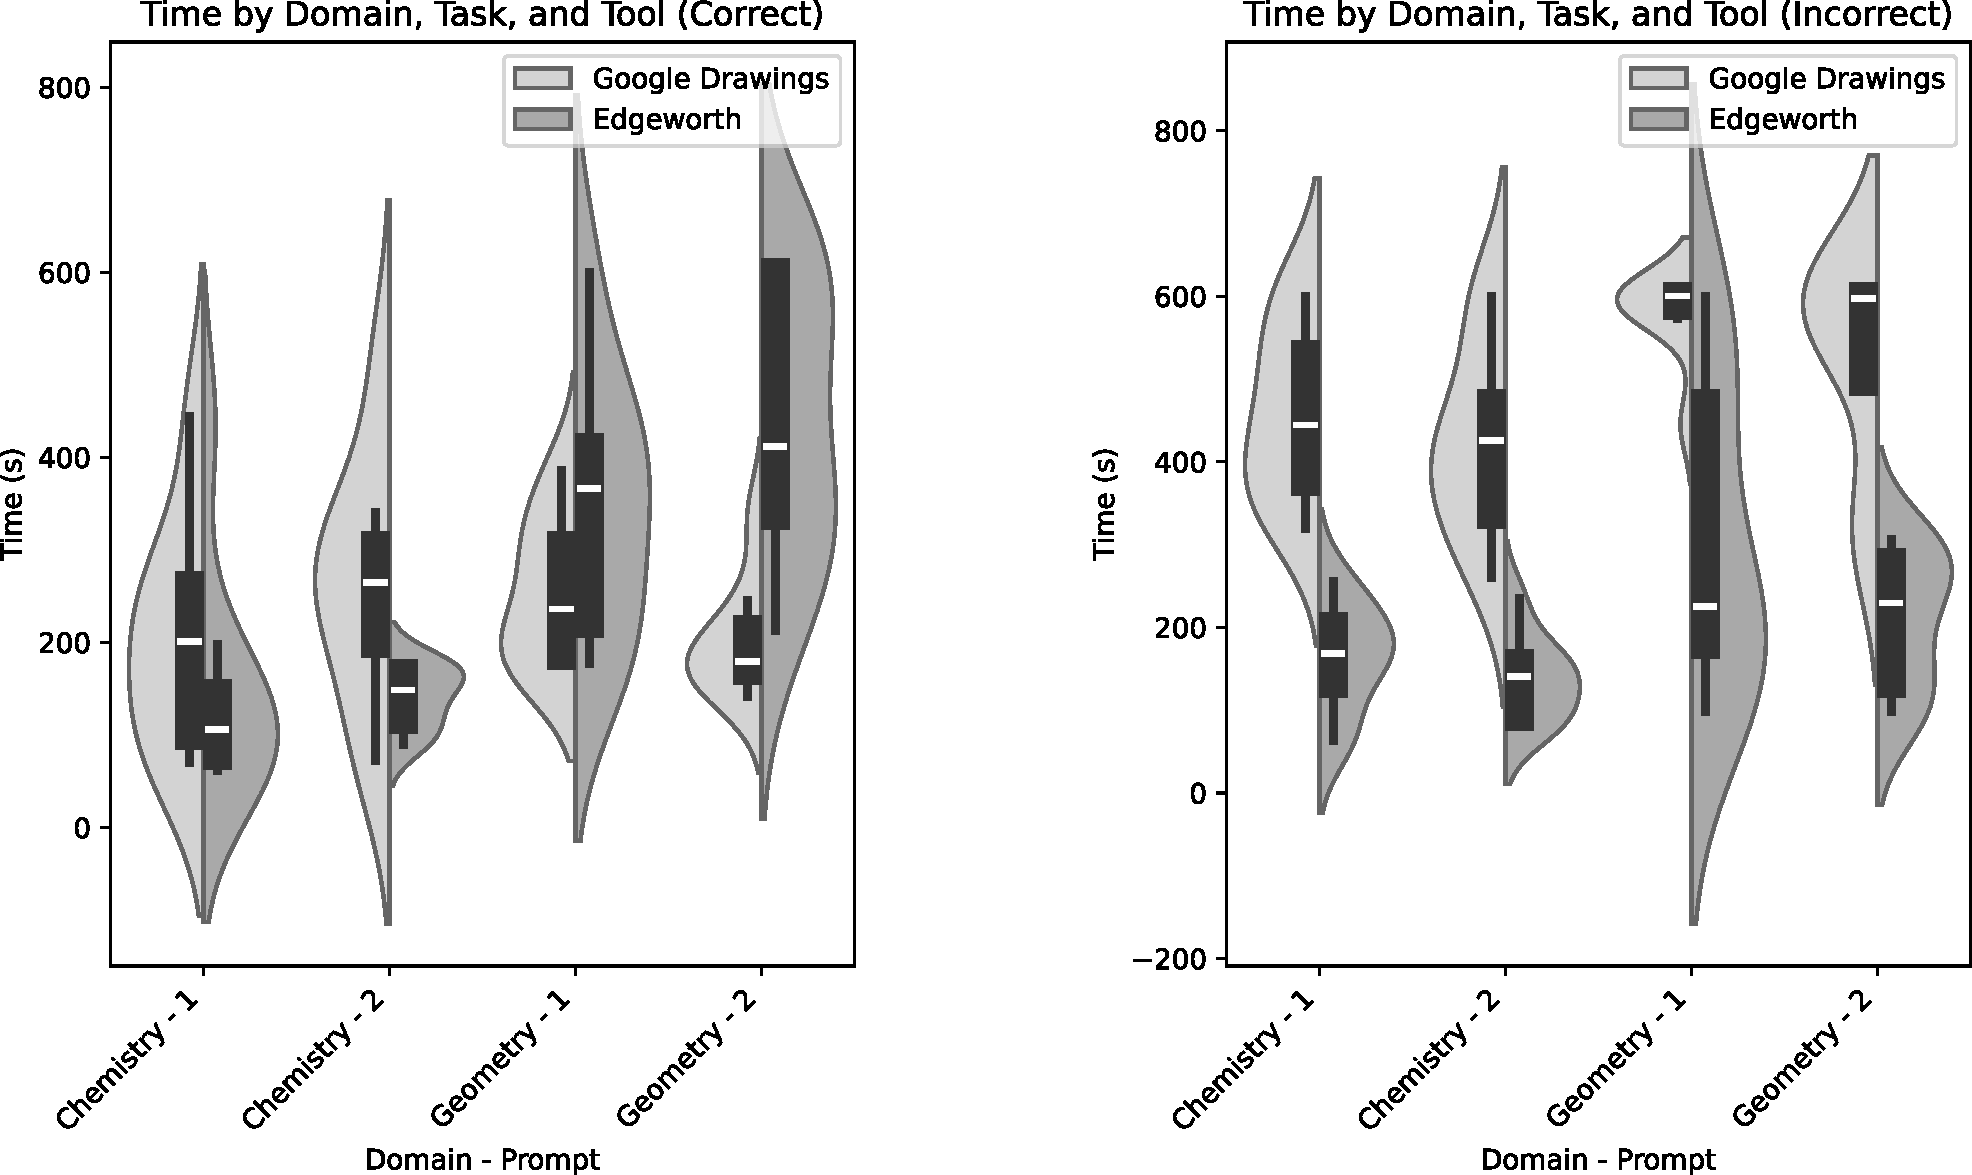
\includegraphics[width=\linewidth]{assets/edgeworth-eval/timing-violin.pdf}
    \caption{Violin plots showing the distribution of time-on-task for both correct (\textbf{Left}) and incorrect (\textbf{Right)} segments of tasks.}
    \label{fig:timing-violin}
\end{figure}


For the incorrect subtasks, the analysis revealed significant differences in task completion times between the tools used, visualized in \cref{fig:timing-violin} \textbf{Right}. In the chemistry domain, participants completed tasks significantly faster (almost 3 times faster) using \Edgeworth (\textit{M} = 150.13s, \textit{SD} = 59.15s) compared to Google Drawings (\textit{M} = 440.63s, \textit{SD} = 113.04s), as indicated by the significant main effect of tool, $F(1, 7) = 53.33, p = 0.0002$. There was no significant effect of the task itself, $F(1, 7) = 1.29, p = 0.293$, suggesting that the difficulty of the tasks was consistent regardless of the tool used. Similarly, in the geometry domain, participants also completed tasks significantly faster (similarly, almost 3 times faster) with \Edgeworth (\textit{M} = 257.25s, \textit{SD} = 139.55s) compared to Google Drawings (\textit{M} = 549.38s, \textit{SD} = 91.28s), with a significant effect of the tool, $F(1, 7) = 90.97, p < 0.0001$. There was a marginal effect of task, $F(1, 7) = 3.64, p = 0.098$, indicating a trend towards task differences that did not reach statistical significance. 

For the correct subtasks, the analysis showed mixed results on \Penrose's performance depending on the domain, illustrated in \cref{fig:timing-violin} \textbf{Left}. In the chemistry domain, participants completed tasks significantly faster using \Penrose (\textit{M} = 144.19s, \textit{SD} = 79.22s) compared to Google Drawings (\textit{M} = 231.81s, \textit{SD} = 129.78s), as indicated by the significant main effect of tool, $F(1, 7) = 6.65, p = 0.037$. There was no significant effect of the task itself, $F(1, 7) = 0.99, p = 0.353$, suggesting that the difficulty of the tasks was consistent regardless of the tool used. In the geometry domain, however, Google Drawings outperformed \Penrose, with participants completing tasks faster using Google Drawings (\textit{M} = 228.5s, \textit{SD} = 71.74s) compared to \Penrose (\textit{M} = 390.94s, \textit{SD} = 149.74s), as indicated by the significant main effect of tool, $F(1, 7) = 15.95, p = 0.005$. Again, there was no significant effect of the task itself, $F(1, 7) = 0.28, p = 0.611$, indicating that the tasks were of similar difficulty.

% survey

In the per-task survey, summarized in \cref{tab:edgeworth-user-study-survey}, participants provided feedback on the tasks across two domains and both tools. For the chemistry tasks, \Edgeworth was rated highly across all survey items, with participants expressing a strong likelihood of using the problems in their classes (\textit{M} = 4.19), finding them pedagogically useful (\textit{M} = 4.25), and rating the visual quality of the diagrams as excellent (\textit{M} = 4.50). In contrast, Google Drawings received lower ratings in chemistry, particularly in terms of visual quality (\textit{M} = 2.81). In the geometry domain, \Edgeworth also was rated well, with participants finding it useful (\textit{M} = 4.06) and visually acceptable (\textit{M} = 3.38), although the ratings were slightly lower compared to chemistry. Google Drawings in geometry was rated lower across all dimensions, with middling scores for usefulness (\textit{M} = 3.50) and visual quality (\textit{M} = 3.44). Overall, \Edgeworth consistently out-rates Google Drawings, particularly in terms of the visual quality of the diagrams and pedagogical usefulness, especially in the chemistry tasks.



\begin{table}[h!]
\centering
\begin{tabular}{l|l|l|l|l}
\hline
\textbf{Domain} & \textbf{Tool} & \textbf{Would Use} & \textbf{Useful} & \textbf{High Quality} \\ \hline
\multirow{2}{*}{\centering Chemistry} 
    & \Edgeworth
    & \progressbar{4.19} 4.19 & \progressbar{4.25} 4.25 & \progressbar{4.50} 4.50 \\ \cline{2-5}
    & Google Drawings 
    & \progressbar{3.63} 3.63 & \progressbar{3.94} 3.94 & \progressbar{2.81} 2.81 \\ \hline

\multirow{2}{*}{\centering Geometry} 
    & \Edgeworth 
    & \progressbar{3.94} 3.94 & \progressbar{4.06} 4.06 & \progressbar{3.38} 3.38 \\ \cline{2-5}
    & Google Drawings 
    & \progressbar{3.38} 3.38 & \progressbar{3.50} 3.50 & \progressbar{3.44} 3.44 \\ \hline
\end{tabular}
\caption{Survey responses for Chemistry and Geometry tasks using Edgeworth and Google Drawings.}
\label{tab:edgeworth-user-study-survey}
\end{table}


\section{Expert Walkthrough Demonstration and Feedback (\ref{rq:eco})}
\label{sec:expert-feedback}

The intended users of \Edgeworth are educators who create problems. These users are very important to the education system since other teachers make use of their problems. Therefore, we recruited educators who created visual practice problems in multiple domains and educational settings to evaluate ecological validity of \Edgeworth-generated problems (\ref{rq:eco}). While an expert survey may suffice for rating problem quality, we opted for walkthrough demonstration, based on prior research on evaluation methods by \citet{Ledo2018EvaluationResearch}, to gather additional qualitative feedback on the value of having the toolkit in their day-to-day work.

\subsection{Participants and Procedure}
\label{sec:expert-procedure}

We recruited domain expert educators of chemistry, geometry, and graph theory. Experts were invited based on their extensive teaching experience in the domain and past experience in \emph{authoring} diagrammatic content. In contrast to the criteria in the formative study (\cref{sec:edgeworth-formative}), this study selected participants based on their domain-specific expertise in authoring problems. Recruited educators came from a wide range of institutions, including MOOC platforms, liberal arts colleges, community colleges, research universities, and secondary schools. The average teaching experience among the 9 expert educators (E1–E9) was 10.33 years, with a standard deviation of 8.39 years, highlighting a broad range of teaching experience. One of the participants is the author of problems in one of the domains in \cref{sec:edgeworth-case-studies}.
\cref{tab:demographics} summarizes the demographic information for 9 expert educators (E1--9) who participated in the study. 

\begin{table}
    \centering
    \begin{tabular}{l|l|l}
        \textbf{Occupation} & \textbf{Yrs} & \textbf{Domain(s)}    \\
        \hline
        MOOC Course Designer       &  7 & Chemistry           \\ 
        Liberal Arts College Prof. &  4 & Chemistry, Geometry \\
        Community College Prof.    & 30 & Chemistry           \\
        Liberal Arts College Prof. & 11 & Graphs              \\
        Research University Prof.  & 17 & Graphs              \\
        Research University Prof.  &  5 & Graphs              \\
        Middle School Teacher      &  5 & Geometry            \\
        Undergraduate TA           &  3 & Geometry, Graphs    \\
        High School Teacher        & 11 & Geometry, Graphs    \\
    \end{tabular}
    \caption{Demographics of walkthrough demonstration participants.}
    % \Description{A table showing the demographics of participants in walkthrough demonstration sessions. It has four columns labeled: ID, Occupation, Teaching Experience, and Domain(s). The entries are: E1 as a MOOC Course Designer with 7 years in Chemistry, E2 as a Professor at a Liberal Arts College with 4 years in Chemistry and Geometry, E3 as a Professor at a Community College with 30 years in Chemistry, E4 as a Professor at a Liberal Arts College with 11 years in Graphs, E5 as a Professor at a Research University with 17 years in Graphs, E6 as a Professor at a Research University with 5 years in Graphs, E7 as a Middle School Teacher with 5 years in Geometry, and E8 as an Elementary School Tutor and Undergraduate TA with 3 years in Geometry and Graphs.}
    \label{tab:demographics}
\end{table}

Each expert participated in a 60- to 90-minute session via video conferencing, which was recorded with their consent. At the start of each session, we demonstrated the workflow of \Edgeworth end-to-end, as described in \cref{sec:edgeworth-workflow}, on one problem outside of the expert's domain. For the remainder of the session, we asked the expert to evaluate two to four problems sampled from \cref{sec:edgeworth-case-studies} in their domain. Per problem, the expert rated 10 diagram variations based on the categories described in \cref{sec:reliability-method}. In addition, we asked participants to provide more granular feedback on diagram quality. After rating the diagram variations, they were asked to pick diagrams to assemble a four-choice diagrammatic translation problem. After the problem was assembled and shown on the interface, we asked (1) if they would use the problem in their instruction and (2) how they would author the diagram using their own workflow. The full study protocol is included in supporting files.

% \subsection{Existing Problem Authoring and Diagramming Processes}

% % thesis: diagramming is a design problem and experts 

% % use of diagrams
% Experts report a wide range of diagram use such as problem sets (E1, E3, E4, \hl{E9}), worked examples (E2--\hl{9}), tests (E1, E2), and in-class activities (E2, E7). Most experts favor multiple-choice translation problems, especially when \quotei{the class size grows} (E2). A few experts favor free-response questions for better feedback to students but noted the scalability problem with them (E2, E3, E7, \hl{E9}). For instance, E3 pointed out that they \quotei{can't monitor how 75 students are drawing a Lewis structure.} 

% % diagram is hard
% To make diagrams, experts used tools such as Microsoft Powerpoint (E1, E3), LaTeX (E4, E5, E6, E8), InkScape~\cite{bah2011inkscape} (E4), Geogebra~\cite{geogebra5} (E2, E7), \hl{and Desmos}~\cite{desmos} (E9). Similar to prior studies on diagramming tools~\cite{naturalDiagramming}, they reported barriers to using these tools that led to \quotei{painful} (E1, E2, E5, E6, E8) diagramming processes. As a result, if possible, they often fell back to hand-drawn diagrams because they \quotei{take less time} (E1, E4, E6), but E5 noted drawing skill is \quotei{one of the talents I did not have and I wish I did.} High-quality diagrams also take significant crafting to get right. For example, E4 would still \quotei{easily spend a day} on a figure because \quotei{if I start trying to make a perfect vector graphics version of it, it's inevitable. We just go down a rabbit hole of trying to make it look nicer and nicer.} 

\subsection{Ecological Validity of Generated Problems}

Overall, experts were happy with the problems they assembled with \Edgeworth-generated diagrams. Experts (E1--9) indicated that they would use all of the problems they created using \Edgeworth in their coursework. Other experts said they would use \Edgeworth-generated problems \quotei{early in the learning process} (E3) and \quotei{as a warm up exercise at the start of the next lecture} (E4). In addition, the problems can be used to review previously introduced concepts. For example, E3 found the diagram variations that break the octet rule to be useful for \quotei{after you've also introduced expanded octet or non-octet-rule things.} Experts plan to use \Edgeworth-generated problem to \quotei{focus on things that students struggle with} (E3) and when introducing concepts that are \quotei{all about visualization} (E5) such as planarity of graphs. E7 was excited to use problems we created in the expressiveness evaluation (\cref{sec:edgeworth-case-studies}) in their class because they were \quotei{going to be covering everything [on the list].} In addition to just asking students to select correct diagrams, E3 also pointed out that by prompting students to \quotei{tell me what is wrong rather than just which is the correct one,} the problem can be used to \quotei{dive deeper.} Similarly, E4 proposed to use \Edgeworth problems as \quotei{an interactive warm-up for reviewing the last lecture, where students vote on and explain why a diagram is correct.} E7 even plans to use \Edgeworth as \quotei{a creative instead of assessment piece} and \quotei{have the students be the teacher \dots{} playing this role more, they get better at tests, because they understand what the test makers are doing.} 

\subsection{Expert Feedback}

% \subsubsection{Experts provided positive qualitative feedback on \Edgeworth}
% fast and good
Experts reacted positively to \Edgeworth. They found \Edgeworth to be a \quotei{perfect fit} (E1, E6, E8) for generating multiple-choice problems, especially \quotei{low-stake} (E2, E3, E5, E6, E8, E9) quizzes that \quotei{incentivize [students] to keep up with the class} (E8). Experts said the automatic layout of \Edgeworth \quotei{draws things really fast} (E5), \quotei{saves you the time of drawing multiple structures} (E3), and produces \quotei{beautiful} (E4, E7) diagrams. Comparing with their existing tools, \Edgeworth is a \quotei{nice time-saver} (E3) and the translation problems they authored during the session would take an \quotei{enormous amount of work} (E4), \quotei{infinitely longer than this took} (E6).

Notably, experts pointed out that \Edgeworth aids creativity by promoting \quotei{recognition over recall} (E6). Specifically, \Edgeworth helps with \quotei{the thinking about how to come up with the graphs} and simplifies the diagram layout such that \quotei{you just generate some mutations that you click refresh until it looks nice} (E6). E2 liked that \quotei{it can come up with different possibilities than the ones that would be immediately apparent to me.} 

In addition, experts commented that \Edgeworth can enable them to give students more practice. For instance, E4 noted that \quotei{there's a feedback loop where \dots{} if I had a really good tool for generating nice multi-choice questions, then I could envision doing that much more frequently.}  

% Importantly, in the context of student authoring problems themselves, E7 thinks that lowering the barrier of problem authoring help students \quotei{feel they have ownership in their learning as well as sharing their ownership with other students in the class.}

% \subsubsection{Experts used visual selection to express diverse standards on diagram quality}

% When rating diagram mutants, experts agreed with diagram ratings of \cref{sec:reliability-eval}, but expressed unique standards for selecting answer choices (\cref{sec:expert-procedure}). Since experts had different standards, they selected different diagrams to assemble problems. This suggests \Edgeworth's use of visual selection met experts' needs.

% One group of experts (E2, E4, E6, E7, E8, \hl{E9}) preferred to maintain a balanced mix of answer choices, \quotei{at least one that's obviously correct, at least one that's obviously incorrect, and then \dots{} two where you have to think about that a little bit} (E6). One rationale was to \quotei{make sure [the problem] is challenging enough, but also has some things that are accessible to students that haven't completely mastered the material} (E4). Another was to teach \quotei{the process of elimination} (E7, \hl{E9}). Another group of experts (E1, E3, E5) had much higher standards for including a mutant in a multiple-choice problem. For example, E1 preferred problems to contain one correct answer and multiple distractor options that are \quotei{less obvious} such that students won't \quotei{pattern match without looking at the details.}

% % On a problem that E2 accepted 7 out of 10 mutants as good incorrect options, E3 discarded 8 out of 10 because they \quotei{violated the octet rule in egregious or blatantly egregious way.} However, E3 said whether the octet rule can be broken depends on \quotei{where students are in the course.}

% The difference of standards is highly individual. From E2's knowledge of \quotei{colleagues [who] only give difficult distractors} and \quotei{certain profs [who] are legendary for having really hard multiple choice,} they guessed that harder problems \quotei{motivate the students to try harder,} but also pointed out that it \quotei{only works for certain students in my experience.} E3 stated that their choice in diagrams \quotei{hinges upon my perception of whether students will automatically disqualify something,} which they admitted is \quotei{a certain premise or bias.}  In E3's words: \quotei{Wow, it's really tough to \dots{} completely take off the instructor hat.} 

% This comment reflects the concept of \textit{expert blind spot} in learning sciences literature, where experts fail to \quotei{understand the processes of novices who are struggling to understand new ideas during their constructive learning process} ~\cite{expertBlindspot}.

% \subsubsection{Experts selected isomorphic diagrams to build conceptual understanding}

\Edgeworth sometimes produces isomorphic diagrams, \ie diagrams with identical content but different layouts. These diagrams occur when \Edgeworth's mutations have no net impact on the example diagram, \eg the mutator removes an edge from a graph and adds it back. Surprisingly, experts found value in these isomorphic diagrams. 
In their geometry course, E2 said that their textbook's diagrams \quotei{get drawn the same way over and over again. And some students get stuck into thinking that the concept is only communicated when the diagram is drawn [exactly] that way.} When assembling a problem about the $HCN$ molecule, E3 compared two isomorphic variations, and picked one over another because \quotei{it's drawn the opposite \dots which is interesting and I think students are going to get it wrong.}  Similarly, E1 finds isomorphic diagrams to be useful for \quotei{molecules with resonance structures.} 
% However, for simpler molecules, E1 cautioned that might mislead students to think that \quotei{they are different structures when they really are the same.} 
E5 found isomorphic planar graphs to be particularly useful because students find them \quotei{painstaking to visualize when they just started.} E5 planned to use \Edgeworth to \quotei{draw a graph that doesn't look like it could be planar first, but then untangle it to show that the graph is actually planar.}






% \subsection{Pilot}

% To prepare the \Edgeworth prototype for evaluation, I will first evaluate the usability of \Edgeworth by recruiting authors to perform small authoring tasks with the \Edgeworth prototype. For example, the participants may be asked to author a simple diagrammatic translation problem. The goal of this pilot study is to identify missing features, usability problems, and opportunities for simplification. The study may include several rounds with increasingly high-fidelity prototypes. After each round, I will refine the design and implement the next prototype. Here are some possible high-level questions for the study:
% \begin{itemize}
%     \item What are the key design considerations for translation problem authoring? How do they fit with the features of \Edgeworth?
%     \item How do authors prefer to work with \Edgeworth? When do they opt to write a configuration file and generate many diagrams? When do they use the by-example workflow? Do they mix the two workflows?
%     \item How does the experience compare to their existing tools? How can \Edgeworth incorporate useful parts of them? 
% \end{itemize}
